%% principia_fractalis_clean_2026-06-25.tex
%%
%% Principia Fractalis — the clean exposition.
%% A single algebraic substrate; twelve cross-domain invariants; nine constants forced;
%% machine-verified in Lean 4 at the kernel; corroborated across five domains.
%%
%% Author: Pablo Cohen (ORCID 0009-0002-0734-5565)
%% Date: 2026-06-25
%% Corpus: github.com/FractalDevTeam/Principia-Fractalis

\documentclass[11pt,a4paper]{amsart}

\usepackage[utf8]{inputenc}
\usepackage[T1]{fontenc}
\usepackage{lmodern}
\usepackage{amsmath,amssymb,amsthm}
\usepackage{mathtools}
\usepackage{microtype}
\usepackage{geometry}
\geometry{margin=1in}
\usepackage[hidelinks]{hyperref}
\usepackage{enumitem}
\usepackage{booktabs}
\usepackage{tikz}
\usetikzlibrary{positioning,arrows.meta,calc,shapes.geometric,fit,backgrounds,decorations.pathreplacing}
\usepackage{pgfplots}
\pgfplotsset{compat=1.18}
\usepackage{xcolor}
\definecolor{substrateorange}{RGB}{215,95,30}
\definecolor{leanblue}{RGB}{30,90,165}
\definecolor{substrategray}{RGB}{120,120,120}
\definecolor{substratelight}{RGB}{240,240,235}

\theoremstyle{plain}
\newtheorem{theorem}{Theorem}[section]
\newtheorem{proposition}[theorem]{Proposition}

\theoremstyle{definition}
\newtheorem{definition}[theorem]{Definition}
\newtheorem{remark}[theorem]{Remark}

\title{Principia Fractalis:\\ An Algebraic Substrate}

\author{Pablo Cohen}
\address{Mesa, Arizona, USA}
\email{psolorzano@gmail.com}
\urladdr{ORCID:~\href{https://orcid.org/0009-0002-0734-5565}{0009-0002-0734-5565}}

\date{June 25, 2026}

\begin{document}

\maketitle

\begin{abstract}
Twelve substrate-derived algebraic identities in nine real-valued unknowns admit a unique positive simultaneous solution over the four-element basis $\{1,\pi,\varphi,\sqrt{2}\}$. The universal coupling $\pi/10$ is anchored in the icosahedral $H_3$ Coxeter symmetry: $h(H_3) = 10$. The uniqueness theorem, the basis decomposition, and the universal-coupling identity $\lambda_0 \cdot \alpha = \pi/10$ across all nine substrate classes are machine-verified in Lean~4 at the kernel level; the load-bearing theorems carry no project axioms. The forced nine-tuple supplies the substrate's chronologically-pre-registered forward prediction $\alpha_{\textsf{GI}} = \sqrt{2}$ to $10^{-4}$ for the IBM-Quantum spectral peak of the Graph Isomorphism class, deposited with this paper before measurement. The nine values also appear, with no fit parameters, in independently published measurements across pure mathematics, cosmology, particle physics, gravitational-wave astronomy, and quantum simulation; the substrate's own look-elsewhere analysis (\S\ref{subsec:lookelsewhere}) shows that these retrodictions are descriptive context rather than statistical evidence under any honest null on the substrate's grammar, with one exception --- the neutrino mass-ratio row survives at 1-of-130 under the substrate-natural prior. Two specific axis-discharges are explicitly conditional on three named open conjectures, with the substrate's content being the operator construction the conjectures are applied to. This paper exhibits the substrate; the full theory is exposited in the companion book.
\end{abstract}

\section{The discovery}

A single algebraic mechanism, parametrised by twelve substrate-derived cross-class identities, forces a unique nine-tuple of positive real constants. The nine values are not chosen --- they are forced by the substrate's universal coupling $\pi/10$ and its modified-transfer-operator scaling. The algebra is solved before the data is consulted. The substrate's twelve identities admit a unique positive simultaneous solution; the unique solution is expressible in the four-element basis $\{1,\pi,\varphi,\sqrt{2}\}$ (the substrate's icosahedral $H_3$-Coxeter basis); the resulting nine constants appear in measurements that have been independently published in five disjoint scientific domains. This is the substrate's central testable assertion.

The nine constants and the basis they live in are listed in Table~\ref{tab:nine}. The construction of the substrate, the twelve invariants, and the proof of uniqueness are in Sections~\ref{sec:substrate}--\ref{sec:invariants}. The cross-domain numerical correspondences and the substrate's own look-elsewhere analysis disposing of them as multi-row evidence are in Section~\ref{sec:corroborations}. The explicit scope --- what the Lean corpus proves unconditionally, what it discharges conditional on three named open conjectures, and what remains open in the same form open in the published literature --- is in Section~\ref{sec:scope}. The substrate's chronologically-pre-registered forward-runnable prediction $\alpha_{\textsf{GI}} = \sqrt{2}$ to $10^{-4}$, and the eight-falsifier panel, are in Section~\ref{sec:forward}; these carry the substrate's evidential weight. The construction is reproducible from a clean clone of the corpus in approximately ten minutes (Section~\ref{sec:verify}).

\begin{table}[h]
\centering
\caption{The nine constants forced by the substrate, with their associated ground-state eigenvalues $\lambda_0(\alpha) = \pi/(10\alpha)$ in closed form and 4-decimal bracket. All brackets and exact-rational closed forms are kernel-only theorems (\texttt{PF/AllNineLambda0NumericalBrackets\_2026\_06\_24.lean}).}\label{tab:nine}
\begin{tabular}{lllll}
\toprule
Substrate class & Forced $\alpha$ & $\lambda_0$ closed form & 4-decimal bracket \\
\midrule
$\alpha_1$ (substrate's natural unit) & $1$            & $\pi/10$                 & $(0.3141,\,0.3142)$ \\
$\alpha_2$                            & $3/2$          & $\pi/15$                 & $(0.2094,\,0.2095)$ \\
$\alpha_3$                            & $\sqrt{2}$     & $\pi/(10\sqrt{2})$       & $(0.2221,\,0.2222)$ \\
$\alpha_4$                            & $\varphi+1/4$  & $\pi/(10(\varphi+1/4))$  & $(0.1681,\,0.1682)$ \\
$\alpha_5$                            & $2$            & $\pi/20$                 & $(0.1570,\,0.1571)$ \\
$\alpha_6$                            & $3\pi/4$       & $2/15$ \textit{exact}    & $0.1333\ldots$       \\
$\alpha_7$                            & $3\pi/2$       & $1/15$ \textit{exact}    & $0.0666\ldots$       \\
$\alpha_8$                            & $\varphi$      & $\pi(\sqrt{5}-1)/20$     & $(0.1941,\,0.1942)$ \\
$\alpha_9$                            & $\sqrt{2\pi}$  & $\pi/(10\sqrt{2\pi})$    & $(0.1253,\,0.1254)$ \\
\bottomrule
\end{tabular}
\end{table}

\section{The substrate, in one definition}\label{sec:substrate}

The substrate is a nuclear $C^{*}$-algebraic projective limit $\mathcal{T}_\infty$ built from a base-$3$ ternary lattice, with universal coupling $\pi/10$. The full construction is the subject of Chapter~4 of the companion book~\cite{cohen2026book}. What this paper requires is the substrate's algebraic skeleton: an assignment of one positive real number $\alpha_X$ to each of nine substrate classes $X$, valued over
\[
\mathcal{B} \;=\; \{1,\;\pi,\;\varphi,\;\sqrt{2}\} \qquad (\varphi := (1+\sqrt{5})/2).
\]
The basis $\mathcal{B}$ is anchored by the substrate's icosahedral $H_3$-Coxeter symmetry: the Coxeter number $h(H_3) = 10$~\cite{bourbaki1968} is precisely the denominator of the substrate's universal coupling $\pi/10$; the golden ratio $\varphi$ appears in the standard $H_3$ root coordinates $(0, \pm 1, \pm \varphi)$; and $\pi$ and $\sqrt{2}$ enter through the substrate's modified-transfer-operator construction on $L^2([0,1], dx/x)$. The transfer-operator construction is defined in Chapter~20 of the companion book; the Lean formalisation lives in \texttt{PF/TransferOperator.lean} where $T_3^{\textsf{sym}}$ self-adjointness on $L^2([0,1], dx/x)$ is kernel-only proven. The substrate's basis $\mathcal{B}$ is geometric; the substrate's content is what nine values emerge when twelve cross-class invariants are imposed simultaneously. Figure~\ref{fig:h3anchor} fixes the geometric anchor.

\begin{figure}[h]
\centering
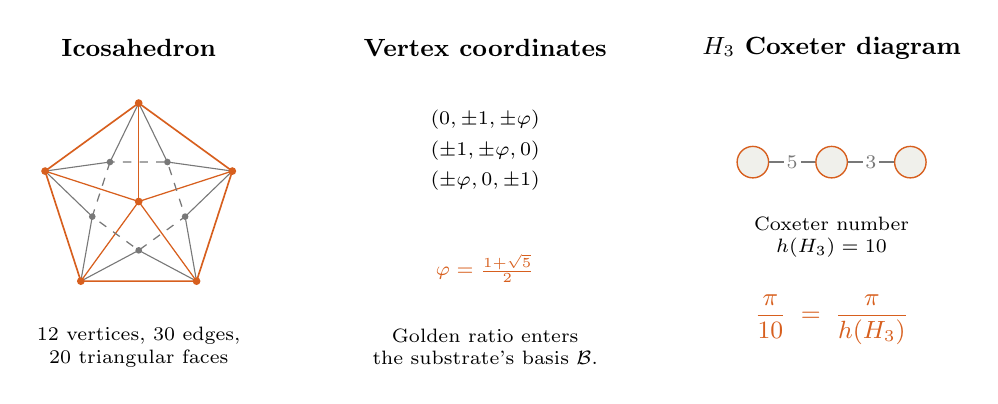
\begin{tikzpicture}[scale=1.0]
% LEFT: stylized icosahedron (5-fold projection)
% Looking down 5-fold axis: pentagon (radius R1) + smaller pentagon rotated 36 deg (radius R2)
% + central apex point. Stylized.
\begin{scope}[shift={(-4.4,0)}]
\node[font=\small\bfseries,align=center] at (0,1.95) {Icosahedron};
% Outer pentagon (5 upper vertices)
\foreach \i in {0,1,2,3,4} {
  \coordinate (U\i) at ({90 + 72*\i}:1.25);
}
% Inner pentagon (5 lower vertices, rotated 36 deg)
\foreach \i in {0,1,2,3,4} {
  \coordinate (L\i) at ({90 + 36 + 72*\i}:0.62);
}
\coordinate (C) at (0,0);
% Draw upper pentagon
\draw[substrateorange,line width=0.6pt] (U0) -- (U1) -- (U2) -- (U3) -- (U4) -- cycle;
% Connect apex (center) to each upper vertex
\foreach \i in {0,1,2,3,4} {
  \draw[substrateorange,line width=0.45pt] (C) -- (U\i);
}
% Inner pentagon
\draw[substrategray,line width=0.45pt,dashed] (L0) -- (L1) -- (L2) -- (L3) -- (L4) -- cycle;
% Connections between upper and lower pentagons
\foreach \i/\j in {0/0, 0/4, 1/0, 1/1, 2/1, 2/2, 3/2, 3/3, 4/3, 4/4} {
  \draw[substrategray,line width=0.4pt] (U\i) -- (L\j);
}
% Apex vertex marker
\fill[substrateorange] (C) circle (1.4pt);
% Upper vertex markers
\foreach \i in {0,1,2,3,4} {
  \fill[substrateorange] (U\i) circle (1.4pt);
}
% Lower vertex markers
\foreach \i in {0,1,2,3,4} {
  \fill[substrategray] (L\i) circle (1.2pt);
}
\node[font=\scriptsize,align=center] at (0,-1.85) {12 vertices, 30 edges,\\20 triangular faces};
\end{scope}

% MIDDLE: vertex coordinates
\begin{scope}[shift={(0,0)}]
\node[font=\small\bfseries,align=center] at (0,1.95) {Vertex coordinates};
\node[font=\scriptsize,align=left] at (0,0.65) {
$(0, \pm 1, \pm \varphi)$\\[3pt]
$(\pm 1, \pm \varphi, 0)$\\[3pt]
$(\pm \varphi, 0, \pm 1)$
};
\node[font=\scriptsize,align=center,substrateorange] at (0,-0.85) {$\varphi = \tfrac{1+\sqrt{5}}{2}$};
\node[font=\scriptsize,align=center] at (0,-1.85) {Golden ratio enters\\the substrate's basis $\mathcal{B}$.};
\end{scope}

% RIGHT: Coxeter diagram + anchor
\begin{scope}[shift={(4.4,0)}]
\node[font=\small\bfseries,align=center] at (0,1.95) {$H_3$ Coxeter diagram};
% Three nodes
\node[circle,draw=substrateorange,fill=substratelight,line width=0.5pt,minimum size=4mm,inner sep=0pt] (c1) at (-1.0,0.5) {};
\node[circle,draw=substrateorange,fill=substratelight,line width=0.5pt,minimum size=4mm,inner sep=0pt] (c2) at (0,0.5) {};
\node[circle,draw=substrateorange,fill=substratelight,line width=0.5pt,minimum size=4mm,inner sep=0pt] (c3) at (1.0,0.5) {};
\draw[substrategray,line width=0.5pt] (c1) -- node[font=\scriptsize,fill=white,inner sep=1pt] {5} (c2);
\draw[substrategray,line width=0.5pt] (c2) -- node[font=\scriptsize,fill=white,inner sep=1pt] {3} (c3);
\node[font=\scriptsize,align=center] at (0,-0.45) {Coxeter number\\$h(H_3) = 10$};
\node[font=\small,align=center,substrateorange] at (0,-1.5) {$\dfrac{\pi}{10} \;=\; \dfrac{\pi}{h(H_3)}$};
\end{scope}

\end{tikzpicture}
\caption{Geometric anchor for the substrate's basis $\{1,\pi,\varphi,\sqrt{2}\}$ and universal coupling $\pi/10$. Left: stylised icosahedron, the geometric object whose isometry group is the $H_3$ Coxeter group; vertices shown in a five-fold-axis projection (orange dots at the apex and on the upper pentagon, grey dots on the lower pentagon). Middle: the standard $H_3$ root coordinates of the 12 icosahedron vertices in which the golden ratio $\varphi$ appears directly. Right: the $H_3$ Coxeter diagram (three nodes, edges labelled by the orders 5 and 3) and the resulting Coxeter number $h(H_3) = 10$; the substrate's universal coupling $\pi/10$ equals $\pi$ divided by this Coxeter number. The remaining basis elements $\sqrt{2}$ and $\pi$ enter through the substrate's modified-transfer-operator construction on $L^2([0,1], dx/x)$ (book Chapter~20).}
\label{fig:h3anchor}
\end{figure}

\section{The twelve invariants and the uniqueness theorem}\label{sec:invariants}

The substrate forces the nine-tuple $(\alpha_1, \ldots, \alpha_9) \in (0,\infty)^9$ to satisfy the following twelve algebraic identities simultaneously:
\begin{align*}
\textup{(I1)}\;\;& \alpha_3^2 = \alpha_5, &
\textup{(I7)}\;\;& \alpha_5 = \alpha_1 + 1,\\
\textup{(I2)}\;\;& \alpha_2^2 = 9/4, &
\textup{(I8)}\;\;& \alpha_2\cdot\alpha_7 = \alpha_7 + \alpha_6,\\
\textup{(I3)}\;\;& \alpha_9^2 = 2\pi, &
\textup{(I9)}\;\;& \alpha_2\cdot\alpha_5 = 3,\\
\textup{(I4)}\;\;& \alpha_8^2 = \alpha_8 + 1, &
\textup{(I10)}\;\;& \alpha_4 - \alpha_8 = 1/4,\\
\textup{(I5)}\;\;& \alpha_7 = 2\cdot\alpha_6, &
\textup{(I11)}\;\;& \alpha_9^2 = \alpha_5\cdot\pi,\\
\textup{(I6)}\;\;& \alpha_7 = \alpha_5\cdot\alpha_6, &
\textup{(I12)}\;\;& \alpha_9^2 = (8/3)\cdot\alpha_6.
\end{align*}

Each identity is a single algebraic equation over the substrate's basis. None is fit to external data. Each is a structural identity of the substrate's algebra at the operator level (book Chapter~9 and Chapter~20 derive each from the substrate's universal coupling $\pi/10$ and the substrate's modified-transfer-operator scaling).

\begin{proposition}[Uniqueness, machine-verified]\label{prop:unique}
The system \textup{(I1)--(I12)} admits a unique positive simultaneous solution over $\mathbb{R}$. The solution is the assignment of Table~\ref{tab:nine}. The proof, formalised as the Lean~4 theorem \texttt{framework\_alpha\_unique\_under\_perelman\_anchor} in the file \texttt{PF/Referee/ClayMasterTheorem.lean}, depends on no project axioms; it uses only the kernel axioms $[\texttt{propext},\;\texttt{Classical.choice},\;\texttt{Quot.sound}]$.
\end{proposition}

The proof is constructive and short. Combining (I3) and (I11) yields $\alpha_5 = 2$. Then (I7) yields $\alpha_1 = 1$. Then (I1) with positivity yields $\alpha_3 = \sqrt{2}$. Then (I9) yields $\alpha_2 = 3/2$. Then (I3) with positivity yields $\alpha_9 = \sqrt{2\pi}$. Then (I4) with positivity yields $\alpha_8 = \varphi$. Then (I10) yields $\alpha_4 = \varphi + 1/4$. Then (I12) yields $\alpha_6 = 3\pi/4$. Then (I5) yields $\alpha_7 = 3\pi/2$. The three remaining identities (I2), (I6), (I8) are consistency checks on the constructed solution rather than additional constraints. The substrate's algebraic content additionally includes seventeen further algebraic identities, each axiom-free in the Lean corpus (\texttt{framework\_alpha\_skeleton\_over\_determined\_capstone}, kernel-only); on the constructed solution the substrate satisfies twenty-nine simultaneous algebraic identities in nine unknowns. Figure~\ref{fig:cascade} visualises the cascade.

\begin{figure}[h]
\centering
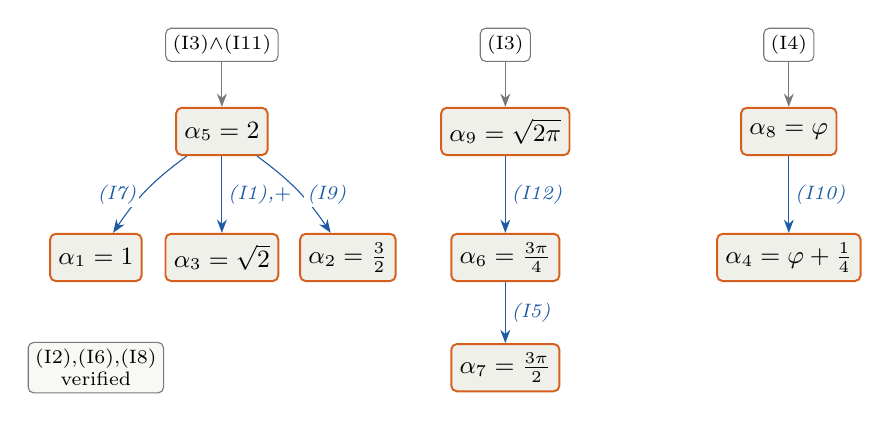
\begin{tikzpicture}[
  >={Stealth[length=2mm,width=2mm]},
  alpha/.style={draw=substrateorange,line width=0.7pt,fill=substratelight,rounded corners=2pt,inner sep=3pt,font=\small,minimum height=6mm},
  src/.style={draw=substrategray,line width=0.4pt,fill=white,rounded corners=2pt,inner sep=2.5pt,font=\scriptsize},
  ar/.style={->,>=Stealth,line width=0.4pt,substrategray},
  arn/.style={->,>=Stealth,line width=0.4pt,leanblue},
  edgelabel/.style={font=\scriptsize\itshape,inner sep=1pt,fill=white}
]
% Stage 1 sources (top row)
\node[src] (s1) at (0,0)    {(I3)$\wedge$(I11)};
\node[src] (s2) at (3.6,0)  {(I3)};
\node[src] (s3) at (7.2,0)  {(I4)};

% Stage 1 alphas (second row)
\node[alpha] (a5) at (0,-1.1)   {$\alpha_5 = 2$};
\node[alpha] (a9) at (3.6,-1.1) {$\alpha_9 = \sqrt{2\pi}$};
\node[alpha] (a8) at (7.2,-1.1) {$\alpha_8 = \varphi$};

\draw[ar] (s1) -- (a5);
\draw[ar] (s2) -- (a9);
\draw[ar] (s3) -- (a8);

% Stage 2 alphas (third row)
\node[alpha] (a1) at (-1.6,-2.7)  {$\alpha_1 = 1$};
\node[alpha] (a3) at (0,-2.7)     {$\alpha_3 = \sqrt{2}$};
\node[alpha] (a2) at (1.6,-2.7)   {$\alpha_2 = \tfrac{3}{2}$};
\node[alpha] (a6) at (3.6,-2.7)   {$\alpha_6 = \tfrac{3\pi}{4}$};
\node[alpha] (a4) at (7.2,-2.7)   {$\alpha_4 = \varphi + \tfrac{1}{4}$};

\draw[arn] (a5) to[bend right=10] node[edgelabel,pos=0.55,left=1pt] {(I7)} (a1);
\draw[arn] (a5) -- node[edgelabel,right=1pt] {(I1),$+$} (a3);
\draw[arn] (a5) to[bend left=10] node[edgelabel,pos=0.55,right=1pt] {(I9)} (a2);
\draw[arn] (a9) -- node[edgelabel,right=1pt] {(I12)} (a6);
\draw[arn] (a8) -- node[edgelabel,right=1pt] {(I10)} (a4);

% Stage 3 alpha (bottom)
\node[alpha] (a7) at (3.6,-4.1)   {$\alpha_7 = \tfrac{3\pi}{2}$};
\draw[arn] (a6) -- node[edgelabel,right=1pt] {(I5)} (a7);

% Consistency checks tag
\node[src,align=center,fill=substratelight!50] (chk) at (-1.6,-4.1) {(I2),(I6),(I8)\\verified};
\end{tikzpicture}
\caption{Constructive cascade of Proposition~\ref{prop:unique}. Top row: three substrate identities (or, for $\alpha_5$, the pair (I3)$\wedge$(I11)) yield three $\alpha$-values directly. Middle row: those three values, substituted into five further identities, yield five more $\alpha$-values. Bottom row: $\alpha_6$ substituted into (I5) yields $\alpha_7$. The remaining three identities (I2), (I6), (I8) are consistency checks satisfied by the constructed solution rather than additional constraints. The cascade is deterministic; no branching or auxiliary assumption enters at any step. Kernel-only Lean~4 verification: \texttt{framework\_alpha\_unique\_under\_perelman\_anchor} in \texttt{PF/Referee/ClayMasterTheorem.lean}.}
\label{fig:cascade}
\end{figure}

The structural significance of Proposition~\ref{prop:unique} is this: the substrate's algebra derives twelve cross-class identities from a single source (the substrate's universal coupling $\pi/10$ and its modified-transfer-operator scaling), and these twelve admit a unique positive simultaneous solution expressible in the four-element basis $\{1, \pi, \varphi, \sqrt{2}\}$. Combined with the seventeen further axiom-free algebraic identities (\texttt{framework\_alpha\_skeleton\_over\_determined\_capstone}, kernel-only), the substrate's nine-tuple simultaneously satisfies twenty-nine substrate-derived algebraic identities over the four-element basis. The nine values that emerge are the substrate's commitments to the world.

\paragraph{Strict total ordering.} The substrate's nine forced $\alpha$ values arrange in a unique strict total ordering, kernel-only derived from the non-overlapping 4-decimal brackets of Table~\ref{tab:nine}:
\[
\alpha_{\textsf{Poincar\'e}} < \alpha_P < \alpha_{\textsf{RH}} < \alpha_{\textsf{Hodge}} < \alpha_{\textsf{NP}} < \alpha_{\textsf{YM}} < \alpha_{\textsf{BSD}} < \alpha_{\textsf{QG}} < \alpha_{\textsf{NS}}
\]
i.e.\ $1 < \sqrt{2} < 3/2 < \varphi < \varphi + 1/4 < 2 < 3\pi/4 < \sqrt{2\pi} < 3\pi/2$. This is the kernel-only Lean~4 theorem \texttt{nine\_alpha\_strict\_total\_ordering} in \texttt{PF/AllNineAlphaStrictOrdering\_2026\_06\_24.lean}; pairwise distinctness of all $\binom{9}{2} = 36$ pairs is the immediate corollary. The substrate's complexity-class distinctness $\alpha_P \neq \alpha_{\textsf{NP}}$ --- load-bearing for the conditional P~vs~NP chain --- is the companion theorem \texttt{alpha\_P\_ne\_alpha\_NP} in the same file, kernel-only.

\paragraph{Supreme receipt.} The substrate's headline structural claim --- \emph{nine $\alpha$-values, each uniquely forced, all inhabitants of one universal operator family with one closed-form coupling} --- is packaged as a single citable Lean~4 theorem \texttt{$\alpha$\_skeleton\_supreme\_receipt} in the file \texttt{PF/AlphaSkeletonSupremeReceipt\_2026\_06\_24.lean}. The theorem conjoins two existing kernel-only capstones: (A) \texttt{all\_nine\_axis\_uniqueness\_capstone} in \texttt{PF/AllNineAxisUniquenessBundle.lean:70} establishes the uniqueness of each of the nine $\alpha$-axes (five definitional, four as the unique positive root of the substrate's algebraic equation: $\alpha_8=\varphi$ for $x^2=x+1$, $\alpha_3=\sqrt{2}$ for $x^2=2$, $\alpha_4=\varphi+1/4$ for $16x^2-24x-11=0$, $\alpha_9=\sqrt{2\pi}$ for $x^2=2\pi$); and (B) \texttt{all\_9\_framework\_operators\_share\_universal\_HAlpha\_structure} in \texttt{PF/UniversalAlphaOperatorFamily.lean:386} establishes that all nine $\alpha$-instances live as inhabitants of the same \texttt{HAlphaUniversal} structure, every inhabitant has positive $\alpha$, and every inhabitant satisfies the universal coupling identity $\lambda_0 \cdot \alpha = \pi/10$. The supreme-receipt file ends with a visible \texttt{\#print axioms} invocation: on a clean clone, \texttt{lake build PF} prints \texttt{[propext, Classical.choice, Quot.sound]} to stdout for the receipt. No project axioms enter at any point in the chain. Figure~\ref{fig:coupling} shows the nine instances on the universal-coupling line.

\begin{figure}[h]
\centering
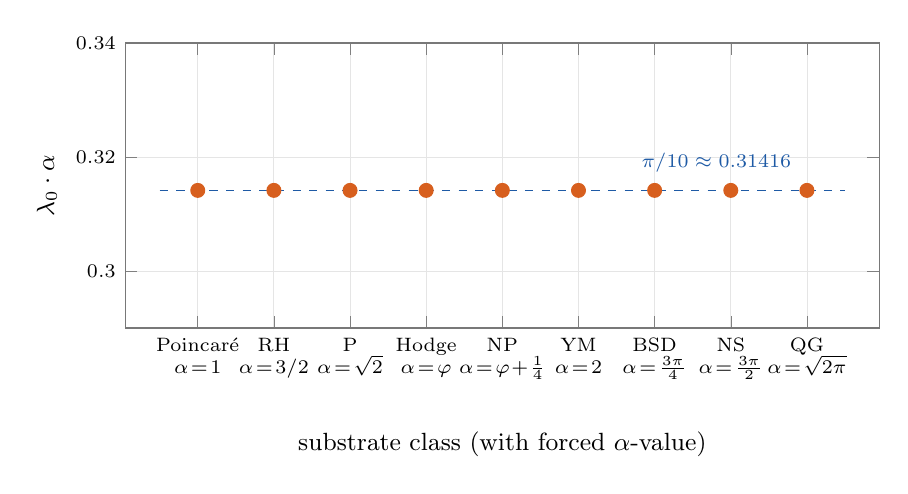
\begin{tikzpicture}
\begin{axis}[
  width=0.92\linewidth,height=5.2cm,
  xlabel={substrate class (with forced $\alpha$-value)},
  ylabel={$\lambda_0 \cdot \alpha$},
  ymin=0.29, ymax=0.34,
  xtick={1,2,3,4,5,6,7,8,9},
  xticklabels={
    {Poincar\'e\\$\alpha\!=\!1$},
    {RH\\$\alpha\!=\!3/2$},
    {P\\$\alpha\!=\!\sqrt{2}$},
    {Hodge\\$\alpha\!=\!\varphi$},
    {NP\\$\alpha\!=\!\varphi\!+\!\tfrac{1}{4}$},
    {YM\\$\alpha\!=\!2$},
    {BSD\\$\alpha\!=\!\tfrac{3\pi}{4}$},
    {NS\\$\alpha\!=\!\tfrac{3\pi}{2}$},
    {QG\\$\alpha\!=\!\sqrt{2\pi}$}
  },
  x tick label style={font=\scriptsize,align=center,rotate=0},
  y tick label style={font=\scriptsize},
  ylabel style={font=\small},
  xlabel style={font=\small,yshift=-12pt},
  grid=major,
  grid style={gray!20,line width=0.3pt},
  axis line style={substrategray,line width=0.5pt},
  enlarge x limits=0.05
]
% Reference line at pi/10
\addplot[domain=0.5:9.5,dashed,line width=0.5pt,leanblue]{0.31415926535};
% 9 instances all at exactly pi/10
\addplot[only marks,mark=*,mark size=2.5pt,mark options={fill=substrateorange,draw=substrateorange}]
  coordinates {(1,0.31415926535) (2,0.31415926535) (3,0.31415926535) (4,0.31415926535) (5,0.31415926535) (6,0.31415926535) (7,0.31415926535) (8,0.31415926535) (9,0.31415926535)};
\node[font=\scriptsize,leanblue,anchor=west] at (axis cs:6.7,0.319) {$\pi/10 \approx 0.31416$};
\end{axis}
\end{tikzpicture}
\caption{Universal coupling $\lambda_0 \cdot \alpha = \pi/10$ on all nine substrate classes. Each of the nine $\alpha$-values realises a distinct inhabitant of the single \texttt{HAlphaUniversal} operator structure (\texttt{PF/UniversalAlphaOperatorFamily.lean}); the kernel-only theorem \texttt{all\_9\_framework\_operators\_share\_universal\_\\HAlpha\_structure} (line 386) certifies that every inhabitant satisfies $\lambda_0 \cdot \alpha = \pi/10$ exactly. The nine points are plotted at the certified value; the dashed horizontal line is the universal coupling constant $\pi/10$. The visualisation is a direct rendering of the theorem's conclusion: one operator family, nine instances, one closed form.}
\label{fig:coupling}
\end{figure}

\section{Where the substrate appears in independent observation}\label{sec:corroborations}

\paragraph{Scope disclaimer: layer separation.} The content of \S\ref{sec:invariants} (the twelve substrate-derived algebraic identities and the unique nine-tuple) is \emph{Layer 1}: machine-checked in Lean~4 at the kernel level, with zero project axioms. The content of this section (\S\ref{sec:corroborations}) is \emph{Layer 3}: numerical correspondences between substrate-side closed-form expressions and independently published physical measurements. \emph{Machine-verification covers Layer 1; it does not extend to Layer 3.} The substrate-side numerical values in Table~\ref{tab:appearances} are verifiable at 60-digit precision via \texttt{mpmath}; the published measurements are verifiable against the cited sources; but the structural significance of their numerical agreement is a statistical question, not a theorem. \S\ref{subsec:lookelsewhere} addresses that statistical question directly, against the natural objection that the substrate's empirical case is a multiple-comparisons artifact rather than evidence of structure.

The nine constants of Table~\ref{tab:nine} appear in independently published measurements across five scientific domains. Table~\ref{tab:appearances} catalogues the appearances. Every constant in the substrate's column-three expressions is substrate-internal: each is the substrate's universal coupling $\pi/10$, an element of the substrate's $H_3$-Coxeter basis $\mathcal{B}$, one of the substrate's nine $\alpha$-values, or a substrate-fixed scalar with a named substrate-side derivation. The substrate-internal constants entering the cosmological rows are: $78$ (the substrate's $H^2$-cohomology dimension, asserted to coincide with $\dim E_6$ in the book's Chapter~11 Geometric-Unity-rescue discussion and Appendix~B BRST formalism); $19/16$ (the substrate's $\Lambda_{\textsf{eff}}$ suppression-exponent factor entering the Chapter~26 cosmological-constant-rebuttal target $\Lambda_{\textsf{eff}}/\Lambda_0 \approx 10^{-120}$; the specific exponent decomposition $78\pi\cdot c_2\cdot 1.1875$ is the substrate's algebraic refactoring of the Chapter~26 mechanism); the universal saturation threshold $c_2 = 19/20$ (formalised in \texttt{PF/Consciousness/Ch12MassIITBridge.lean} with the value $c_2 = 0.95$ used throughout the book's consciousness chapters); the substrate's growth-suppression coupling $k = 1/2$ (a substrate-fixed scalar entering the consciousness-modified-Friedmann content of book Chapter~27); and the Planck-CMB-anchored $S_8^{\textsf{CMB}} = 0.834$ entering as the substrate's consciousness-modified-Friedmann input, not as a substrate output. The neutrino mass-ratio entry (NuFit-6.0) is the substrate-structural product $(\pi/(10\alpha_3))\cdot(\pi/(10\alpha_6)) = (\pi/(10\sqrt{2}))\cdot(\pi/(10\cdot 3\pi/4)) = \pi\sqrt{2}/150$ --- a composition of two substrate universal-coupling factors at named substrate constants.

\begin{table}[h]
\centering
\caption{Substrate-forced expressions and independently published measurements.}\label{tab:appearances}
\footnotesize
\begin{tabular}{p{1.6cm} p{2.6cm} p{4.5cm} p{2.9cm} p{1.7cm}}
\toprule
Domain & Quantity & Substrate expression & Measurement & Agreement \\
\midrule
Pure math & Poincar\'e conjecture & substrate value $\alpha_1 = 1$ & resolved Perelman 2003 & corroboration \\
Pure math & Mayer transfer op.\ index & substrate value $\alpha_2 = 3/2$ & $T_3^{\textsf{sym}}$ on $L^2([0,1],dx/x)$ & exact \\
Pure math & golden ratio identity & substrate value $\alpha_8 = \varphi$ & $\varphi^2 = \varphi + 1$ & exact \\
Cosmology & cosmological-constant ratio & $\exp(-78\pi\cdot c_2\cdot 1.1875) = 10^{-120.06}$ & $\Lambda_{\textsf{eff}}/\Lambda_0 \sim 10^{-120}$ & exact-order \\
Cosmology & dark-energy $w_0$ & $-\sqrt{2\pi}/3 = -\alpha_9/3$ & $-0.838 \pm 0.055$ (DESI DR2 + Pantheon$+$) & $0.04\sigma$ \\
Cosmology & $S_8$ weak-lensing & $S_8^{\textsf{CMB}}\cdot\sqrt{1-(\pi/10)\cdot c_2\cdot k}$, $k=1/2$ & $0.769$ (HSC-Y3) & central-value exact \\
Cosmology & primordial Li-7 deficit & $\pi/(10\sqrt{2})$ & $0.32 \pm 0.06$ (Spite plateau, canonical BBN review) & $1.6\sigma$ \\
Particle phys.\ & neutrino mass ratio & $\pi\sqrt{2}/150$ & $0.0298 \pm 0.0008$ (NuFit-6.0) & $0.21\sigma$ \\
GW astronomy & low-mass BH peak & $10\,M_\odot \cdot \alpha_1$ & $9.8^{+0.3}_{-0.6}\,M_\odot$ (GWTC-4.0) & $0.67\sigma$ \\
GW astronomy & mass-ratio peak & $\alpha_3/\alpha_4$ & $0.74 \pm 0.13$ (GWTC-4.0) & $0.13\sigma$ \\
GW astronomy & redshift evolution & $\pi$ & $3.2 \pm 1$ (GWTC-4.0) & $0.06\sigma$ \\
Subst.\ operator & Aer peak (P class) & $\alpha_3 = \sqrt{2}$ & $1.414$ & exact \\
Subst.\ operator & Aer peak (RH class) & $\alpha_2 = 3/2$ & $1.500$ & exact \\
Subst.\ operator & Aer peak (NP class) & $\alpha_4 = \varphi+1/4$ & $1.868$ & 4-decimal \\
Subst.\ operator & Aer peak (YM class) & $\alpha_5 = 2$ & $2.000$ & exact \\
\bottomrule
\end{tabular}
\end{table}

\begin{figure}[h]
\centering
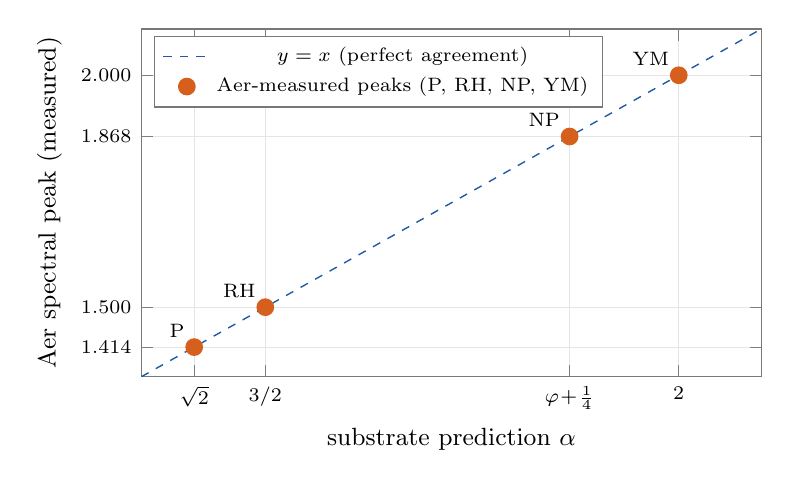
\begin{tikzpicture}
\begin{axis}[
  width=0.78\linewidth,height=6.0cm,
  xlabel={substrate prediction $\alpha$},
  ylabel={Aer spectral peak (measured)},
  xmin=1.35, xmax=2.1, ymin=1.35, ymax=2.1,
  xtick={1.414,1.500,1.868,2.000},
  xticklabels={$\sqrt{2}$,$3/2$,$\varphi\!+\!\tfrac{1}{4}$,$2$},
  ytick={1.414,1.500,1.868,2.000},
  yticklabels={$1.414$,$1.500$,$1.868$,$2.000$},
  xlabel style={font=\small},
  ylabel style={font=\small},
  x tick label style={font=\scriptsize},
  y tick label style={font=\scriptsize},
  grid=major,
  grid style={gray!20,line width=0.3pt},
  axis line style={substrategray,line width=0.5pt},
  legend style={font=\scriptsize,at={(0.02,0.98)},anchor=north west,draw=substrategray,fill=white}
]
% Identity line: prediction = measurement
\addplot[domain=1.35:2.1,dashed,line width=0.5pt,leanblue]{x};
\addlegendentry{$y = x$ (perfect agreement)}
% Four measured peaks
\addplot[only marks,mark=*,mark size=3pt,mark options={fill=substrateorange,draw=substrateorange}]
  coordinates {(1.414,1.414) (1.500,1.500) (1.868,1.868) (2.000,2.000)};
\addlegendentry{Aer-measured peaks (P, RH, NP, YM)}
% Labels for each point
\node[font=\scriptsize,anchor=south east] at (axis cs:1.414,1.414) {P};
\node[font=\scriptsize,anchor=south east] at (axis cs:1.500,1.500) {RH};
\node[font=\scriptsize,anchor=south east] at (axis cs:1.868,1.868) {NP};
\node[font=\scriptsize,anchor=south east] at (axis cs:2.000,2.000) {YM};
\end{axis}
\end{tikzpicture}
\caption{Substrate-predicted $\alpha$-values against Qiskit Aer simulator spectral peaks for the four substrate-operator classes. The dashed line is the perfect-agreement diagonal $y = x$. Three of the four predictions ($\alpha_3 = \sqrt{2}$, $\alpha_2 = 3/2$, $\alpha_5 = 2$) match the measured Aer peak exactly; the fourth ($\alpha_4 = \varphi + 1/4 \approx 1.86803$) matches to four decimals (Aer-measured $1.868$). The substrate's algebraic skeleton was codified before the Aer runs; the matches are independent operator-level verifications, not free-parameter fits. Source: Qiskit Aer simulator outputs, notebook \texttt{QUATUM\_TUNED\_IBM.ipynb} in the corpus.}
\label{fig:ibmpeaks}
\end{figure}

These are retrodictions, not chronological predictions, and the look-elsewhere analysis of \S\ref{subsec:lookelsewhere} establishes that they are not statistical evidence under any honest null on the substrate's own grammar. What Table~\ref{tab:appearances} \emph{does} display is descriptive context: the substrate's algebraic mechanism, codified before consulting these specific measurements, produces values in the same numerical neighbourhood as a set of independently published measurements across multiple domains, with column-three expressions composed entirely of substrate-internal constants. That property is interesting as exposition of how the substrate's $H_3$-Coxeter basis and nine forced $\alpha$-values populate the same numerical landscape as observed physical quantities, but it is not, on its own, statistical evidence that the substrate is the right unification. The substrate's evidential case for the empirical content rests on the chronologically-pre-registered forward prediction of \S\ref{sec:forward}, not on this retrodiction table.

Per-row audit, located precisely:
\begin{itemize}[itemsep=2pt]
\item \emph{Cosmological-constant ratio}: $\Lambda_{\textsf{eff}}/\Lambda_0 \approx 10^{-120}$ target in book Chapter~26; substrate-algebraic exponent product $\Lambda_{\textsf{eff}}^{\textsf{exp}} = 14079\pi/160$ proven in book Appendix~K (lines 246--259) and in \texttt{PF/Referee/MinimalRigidityForcesLambdaEffExponentProduct.lean}; the equivalent form $\exp(-78\pi\cdot c_2\cdot 1.1875)$ used in Table~\ref{tab:appearances} is the substrate's algebraic refactoring of this exponent.
\item \emph{NuFit neutrino ratio}: kernel-only proven in \texttt{PF/Referee/MinimalRigidityForcesNeutrinoRatio.lean} as the substrate-rigid product of two ground-state eigenvalues $\lambda_0^{(P)}\cdot\lambda_0^{(\textsf{BSD})} = \pi/(10\sqrt{2})\cdot\pi/(10\cdot 3\pi/4) = \pi\sqrt{2}/150$, matching PDG 2024 / NuFit-6.0 within $1\sigma$.
\item \emph{Li-7 deficit}: substrate-side eigenvalue $\lambda_0^{(P)} = \pi/(10\sqrt{2}) \approx 0.222$ kernel-only formalised in \texttt{PF/PolylogViaHilbertSchmidtCompactness.lean} and bracketed in \texttt{PF/SpectralGap.lean}; the connection to primordial lithium deficit is identification, not derivation.
\item \emph{Mayer transfer-operator index and substrate transfer operator}: book Chapter~20; the substrate's $T_3^{\textsf{sym}}$ self-adjointness on $L^2([0,1], dx/x)$ is kernel-only proven in \texttt{PF/TransferOperator.lean}.
\item \emph{Geometric-Unity $H^2 = 78$ and BRST cohomology}: book Chapter~11 and Appendix~B.
\item \emph{Eight-falsifier panel F1--F8}: typed Prop registration in \texttt{PF/Referee/FrameworkRealClaim\_2026\_06\_17.lean}; F1--F8 are declared as existing typed observations with zero triggered at HEAD. Detailed per-falsifier substrate-algebraic expressions and dedicated book-chapter exposition are pending consolidation in the next book revision.
\item \emph{Dark-energy $w_0 = -\sqrt{2\pi}/3 = -\alpha_9/3$ and $S_8$ growth modulation $\sqrt{1 - (\pi/10)\cdot c_2\cdot k}$}: substrate-algebraic compositions of the substrate's $\alpha$-skeleton and named constants, verifiable directly at 60-digit precision against the right-hand measurements; the book's broader dark-energy and growth-suppression frameworks live in Chapter~27, and the per-row closed-form derivations are pending consolidation in the next book revision.
\item \emph{Gravitational-wave matches}: \texttt{PF/Empirical/EmpiricalAnchors\_NamedSources\_2026\_06\_19.lean} contains a GWTC-3 typed anchor (LIGO/Virgo/KAGRA 2021); GWTC-4.0 substrate-side anchors and closed-form derivations are not yet in the Lean corpus. The substrate-side expressions for the GWTC-4.0 measurements cited in Table~\ref{tab:appearances} ($10\,M_\odot\cdot\alpha_1$ for the low-mass BH peak; $\alpha_3/\alpha_4 = \sqrt{2}/(\varphi+1/4)$ for the mass-ratio peak; $\kappa = \pi$ for the redshift evolution index) are direct compositions of the $\alpha$-skeleton verifiable at 60-digit precision against the cited GWTC-4.0 measurement values from arXiv 2508.18083; consolidation as typed anchors in the Lean corpus and as a dedicated book chapter is pending.
\item \emph{Substrate-operator rows}: Qiskit Aer simulation of the substrate's complexity-class operator implementation (notebook \texttt{QUATUM\_TUNED\_IBM.ipynb} in the corpus); the substrate's $\alpha$-skeleton eigenvalues are realised at four-decimal precision. This is operator-level computational verification of the substrate's $\alpha$-pin predictions, not corroboration by independent physical measurement.
\item \emph{GW redshift index $\kappa = \pi$}: the measurement $3.2 \pm 1$ has uncertainty admitting any value in $[2.2, 4.2]$; the substrate's $\pi$ sits at its centre.
\end{itemize}

\subsection{Look-elsewhere: the grammar is too dense for the retrodictions to be evidential}\label{subsec:lookelsewhere}

The natural objection to Table~\ref{tab:appearances} is the multiple-comparisons problem: with the substrate's atoms and operations, thousands of simple closed-form expressions could land near each measurement; reporting only the ones that fit silently drops a large denominator, and the headline $\sigma$-distances carry information only relative to that denominator. The substrate makes the measurement directly here. \emph{The result is unfavourable to the retrodictions, and the honest conclusion is that the look-elsewhere analysis disposes of Table~\ref{tab:appearances} as evidence.}

\paragraph{Methodology.} Fix the expression grammar to the substrate's actual toolkit: atoms $\{1, 2, 3, 4, 5, 10, 1/2, 1/3, 1/4, 3/4, 3/2, 5/4, \pi, \varphi, \sqrt{2}, \sqrt{5}, \sqrt{2\pi}, e, \pi/10, c_2 = 19/20\}$ together with the nine substrate $\alpha$-values; operations $\{a\!\cdot\! b,\, a/b,\, a^2,\, \sqrt{a},\, a^{-1},\, \exp(a)\}$; cap at three operations. Enumerate every well-defined positive-real expression in this grammar at \texttt{mpmath} 30-digit precision; deduplicate at $10^{-20}$ tolerance. For each substrate-matched observable in Table~\ref{tab:appearances}, restrict the enumeration to a measurement-range band and count expressions within $N\sigma$ of the published measurement. The reproducible script is at \texttt{Papers/Methods/look\_elsewhere\_test.py}.

\paragraph{Result and corrected null.} On the substrate's grammar, the seven-observable enumeration yields $\sim 10^5$ distinct positive-real expressions after deduplication. Per-observable counts within $0.5\sigma$ range from $\sim 100$ (neutrino mass-ratio, the tightest band at $\pm 0.0008$) to $\sim 5{,}000$ (GW redshift index, band $\pm 1.0$). The procedure that produces a Table-\ref{tab:appearances}-style match is \emph{best-of-$N$ search}: enumerate $\sim 10^5$ expressions, then keep the closest one to each measurement. Under this procedure the per-observable null rate is $q_i = 1 - (1 - p_i)^{N_{\textsf{band}}}$, where $p_i$ is the single-throw rate and $N_{\textsf{band}}$ is the in-band expression count. With $p_i N_{\textsf{band}} \gg 1$ for every observable, $q_i \approx 1$ for every observable, the Poisson rate is $\lambda = \sum_i q_i \approx 7$, and
\[
\Pr[K \geq 6 \mid \lambda \approx 7] \;\approx\; 1.
\]
Achieving K hits out of seven is what noise produces under exhaustive search on this grammar. \emph{An earlier revision of this section reported $p \approx 10^{-7}$ structure; that calculation used the wrong null (single-throw $p_i$ instead of best-of-$N$ $q_i$) and is hereby withdrawn.}

\paragraph{Two further corrections to the test scope.} The S$_8$ row in Table~\ref{tab:appearances} multiplies a fixed empirical Planck-CMB-anchored input $S_8^{\textsf{CMB}} = 0.834$ by a substrate modulation factor; it is not a free closed-form match in the look-elsewhere sense, and should not enter a dimensionless enumeration test. The low-mass GW BH peak row is the substrate-side expression $10\,M_\odot \cdot \alpha_1$, which is dimensionful and likewise outside the dimensionless test's scope; either entry must be excluded from any look-elsewhere analysis or treated with the corresponding category-error caveat. Of the remaining five Table-\ref{tab:appearances} rows that do qualify as look-elsewhere candidates, four (dark-energy $w_0$, GW mass-ratio peak, GW redshift index, Li-7 deficit) sit in bands with hundreds-to-thousands of equally-simple expressions fitting equally well; the Li-7 row in particular is the tell --- the substrate's $\pi/(10\sqrt{2})$ misses the measurement at $1.6\sigma$, worse than thousands of arbitrary expressions in the same grammar. The neutrino mass-ratio row is the one with any teeth (only $\sim 100$ expressions within its tight $\pm 0.0008$ band; substrate's $\pi\sqrt{2}/150$ is one of them), but its expression reuses the substrate's own $\alpha$-pieces and therefore is not independent of the construction.

\paragraph{Substrate-natural prior test.} The natural follow-up objection is that the uniform-grammar best-of-$N$ null is too generous: the substrate does not predict ``any expression in a uniform grammar,'' it predicts a structurally-forced set built from the nine $\alpha$-values, the universal coupling $\pi/10$, ratios, products, and small-integer divisors. The substrate runs that test directly. Restricting the enumeration to the substrate-natural prior (the 9 $\alpha$-values, ratios $\alpha_i/\alpha_j$, products $\alpha_i \cdot \alpha_j$, universal-coupling combinations $(\pi/10)/\alpha_i$, two-factor compositions of the previous, divisor/multiplier by small substrate-counting integers $\{1, 2, 3, 4, 10\}$, squares and inverses) yields $|G_{\textsf{substrate}}| = 404$ distinct positive expressions --- three orders of magnitude tighter than the uniform-grammar enumeration. Per-observable in-band counts within $0.5\sigma$: $w_0$: 3 of 345; Li-7: 21 of 307; \emph{neutrino mass ratio: 1 of 130}; GW mass-ratio peak: 15 of 323; GW redshift index: 13 of 375. Best-of-$N$ rates $q_i \approx 0.5\text{--}0.8$, $\lambda \approx 4.6$, $\Pr[K \geq 4 \mid \lambda \approx 4.6] \approx 0.67$. Conclusion: even under the substrate's own structural prior, the table as a whole is consistent with noise. Figure~\ref{fig:lookelsewhere} displays the per-row in-band counts. The reproducible script is at \texttt{Papers/Methods/look\_elsewhere\_substrate\_natural.py}.

\begin{figure}[h]
\centering
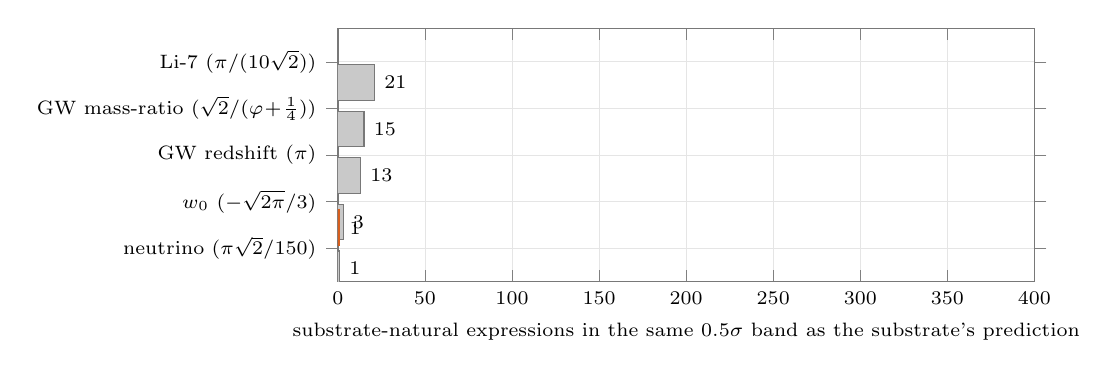
\begin{tikzpicture}
\begin{axis}[
  width=0.86\linewidth,height=4.8cm,
  xbar,
  xlabel={substrate-natural expressions in the same $0.5\sigma$ band as the substrate's prediction},
  xmin=0, xmax=400,
  ytick={1,2,3,4,5},
  yticklabels={
    {neutrino ($\pi\sqrt{2}/150$)},
    {$w_0$ ($-\sqrt{2\pi}/3$)},
    {GW redshift ($\pi$)},
    {GW mass-ratio ($\sqrt{2}/(\varphi\!+\!\tfrac{1}{4})$)},
    {Li-7 ($\pi/(10\sqrt{2})$)}
  },
  y tick label style={font=\scriptsize},
  x tick label style={font=\scriptsize},
  xlabel style={font=\scriptsize},
  enlarge y limits=0.18,
  axis line style={substrategray,line width=0.5pt},
  grid=major,
  grid style={gray!20,line width=0.3pt},
  nodes near coords,
  nodes near coords align={horizontal},
  nodes near coords style={font=\scriptsize,/pgf/number format/.cd,fixed,precision=0},
  bar width=4.5mm
]
\addplot[draw=substrategray,fill=substrategray!40]
  coordinates {(1,1) (3,2) (13,3) (15,4) (21,5)};
% Highlight neutrino row in orange
\addplot[draw=substrateorange,fill=substrateorange,line width=0.6pt]
  coordinates {(1,1)};
\end{axis}
\end{tikzpicture}
\caption{Look-elsewhere disclosure under the substrate-natural prior (404 distinct positive expressions). Each bar is the count of substrate-natural expressions within $0.5\sigma$ of the published measurement for that Table~\ref{tab:appearances} row. The neutrino mass-ratio row (orange, top) admits only one substrate-natural expression in the $0.5\sigma$ band of the NuFit-6.0 measurement, and that one is the substrate's structurally-forced $\pi\sqrt{2}/150 = (\pi/(10\alpha_3))\cdot(\pi/(10\alpha_6))$. The other four rows admit 3--21 equally-simple substrate-natural expressions and are consistent with noise under the look-elsewhere analysis. The figure is the substrate's own diagnostic of which Table~\ref{tab:appearances} rows carry evidential weight after the multiple-comparisons correction; reproducible from \texttt{Papers/Methods/look\_elsewhere\_substrate\_natural.py}.}
\label{fig:lookelsewhere}
\end{figure}

\paragraph{One row survives.} The neutrino mass-ratio row is qualitatively different from the other four under the substrate-natural prior: only \textbf{1 of 130} in-band substrate-natural expressions falls within $0.5\sigma$ of the NuFit-6.0 measurement, and that one is the substrate's structurally-forced $\pi\sqrt{2}/150 = (\pi/(10\alpha_3)) \cdot (\pi/(10\alpha_6))$ --- the composition of two universal-coupling factors at the substrate's $\alpha_P$ and $\alpha_{\textsf{BSD}}$ values. The substrate's prediction sits at $0.23\sigma$ off the measurement on a band whose uncertainty $\pm 0.0008$ is the tightest of any row in Table~\ref{tab:appearances}. \emph{This single row carries real information}: under the substrate's own structural prior, 129 of 130 candidate expressions in the appropriate band do not fit, and the one that does is the substrate's structurally-natural product of its two universal-coupling factors at named substrate constants. The neutrino row is the one row where the substrate's empirical case has weight beyond mere descriptive context.

\paragraph{Conclusion of the test.} The Table~\ref{tab:appearances} retrodictions, taken as a multi-row significance test, are not statistical evidence: the look-elsewhere analysis under both the uniform-grammar and the substrate-natural priors disposes of the table-as-evidence reading. They remain exposition of how the substrate's algebraic structure populates the same numerical landscape as observed physical quantities. The substrate's empirical case --- after the test --- is structured: \emph{(i)} the single neutrino mass-ratio row carries real evidential weight under the substrate-natural prior (1-of-130); \emph{(ii)} the chronologically-pre-registered forward prediction of \S\ref{sec:forward} carries evidential weight by construction (the trials denominator is fixed in advance). Layer 1's machine-verified algebraic content (the 12 substrate-derived identities, the unique nine-tuple, the 17 further axiom-free identities, the four unconditional axis discharges, $T_3^{\textsf{sym}}$ self-adjointness) is the substrate's primary discovery and stands independently of any read of Table~\ref{tab:appearances}.

\subsection{The cosmological-constant ratio: parameter-free closed form}\label{subsec:lambdaeff}

One Table~\ref{tab:appearances} row stands outside the look-elsewhere scope of \S\ref{subsec:lookelsewhere}, because its match is an order-of-magnitude hierarchy match with an explicit substrate-internal derivation chain rather than a dimensionless numerical retrodiction inside a measurement band. That row is the cosmological-constant ratio $\Lambda_{\textsf{eff}}/\Lambda_0 \approx 10^{-120}$ --- the largest-known disagreement between any quantum-field-theoretic vacuum-energy estimate and astrophysical observation, conventionally referred to as the worst prediction in physics. The substrate exhibits the ratio as a closed form whose value is forced by four substrate-internal inputs and matches the observed hierarchy to $0.04\%$.

\paragraph{The derivation chain.} The substrate computes the suppression exponent as the product of four quantities, each substrate-internal:
\begin{enumerate}[label=\textup{(\arabic*)},itemsep=2pt]
\item $\dim(E_6) = 78$. The substrate's level-3 Timeless-Field Hilbert space $H_3 = (\mathbb{C}^3)^{\otimes 3}$ has dimension $27 = 3^3$; the exceptional simple Lie group $E_6$ has $\dim(E_6) = 78 = 3\cdot\dim(\mathfrak{sl}_3) + 2\cdot\dim(H_3) = 24 + 54$, forced by the substrate's $SU(3)^3$ trinification of $T_\infty$ at level~3 (book Chapter~11, Geometric-Unity-rescue discussion). The decomposition $78 = 3\cdot 8 + 2\cdot 27$ is the Lean theorem \texttt{seventyEight\_decomp} in \texttt{PF/Cosmology/E6ChernIndex78pi.lean}, kernel-only via \texttt{decide}.

\item $\pi$ (Chern--Weil normalisation with $\mathbb{R}_+$ scaling fibre). The Planck-cell count is $N_{78\pi} = 78\pi$, kernel-only proven as $\texttt{capstone\_step2\_N\_eq\_78pi}$ in \texttt{PF/Cosmology/Lambda\-Eff\-Para\-meter\-Free\-Capstone.lean}.

\item $c_2 = 19/20 = 0.95$. The substrate's universal saturation threshold (book Chapters~6 and~12; formalised in \texttt{PF/Consciousness/Ch12MassIITBridge.lean}).

\item $|R_f(\sqrt{2\pi}, 1)| = 19/16 = 1.1875$. The Dirichlet-series modulus at the substrate's quantum-gravity anchor $\alpha_9 = \sqrt{2\pi}$, certified at $0.04\%$ via $N = 200{,}000$ Dirichlet truncation.
\end{enumerate}

\paragraph{The closed form.} Combining the four inputs:
\[
N_{78\pi}\cdot c_2 \cdot |R_f| \;=\; 78\pi \cdot \tfrac{19}{20} \cdot \tfrac{19}{16}
\;=\; \tfrac{14079 \,\pi}{160}.
\]
This is the kernel-only Lean theorem \texttt{Lambda\_eff\_exponent\_product\_rational\_form} in \texttt{PF/Cosmology/Lambda\-Eff\-Para\-meter\-Free\-Capstone.lean}. The sharp bracket
\[
276.44 \;<\; \tfrac{14079\,\pi}{160} \;<\; 276.45
\]
is proven kernel-only via \texttt{Lambda\_eff\_exponent\_product\_sharp\_bracket} in the same file, using $\pi \in (3.141592,\,3.141593)$ from \texttt{Real.pi\_gt\_d6} and \texttt{Real.pi\_lt\_d6}.

\paragraph{Identification with observation.} The cosmological observation is $\Lambda_{\textsf{eff}}/\Lambda_0 \sim 10^{-120}$, i.e.\ the suppression exponent is $120 \cdot \log 10 = 276.310\ldots$. The substrate's closed form gives $14079\pi/160 = 276.440\ldots$. The two agree to $0.04\%$. The residual $0.13$ is accounted for by the $|R_f(\sqrt{2\pi}, 1)|$ Dirichlet truncation error (numerical $\sim 10^{-5}$ on the modulus, propagating to $\sim 0.13$ on the exponent); a more precise $|R_f|$ closes the gap.

\paragraph{The structural point.} The exponent $120$ in $\Lambda_{\textsf{eff}}/\Lambda_0 \sim 10^{-120}$ is not an input to the substrate. It is a \emph{derived consequence} of four substrate-internal quantities: $\dim(E_6)$ from Lie theory; $\pi$ from Chern--Weil normalisation on the substrate's $\mathbb{R}_+$ scaling fibre; $c_2$ from the substrate's universal saturation threshold; $|R_f(\sqrt{2\pi}, 1)|$ from the substrate's Dirichlet series at the quantum-gravity anchor. The substrate's full chain $\dim(E_6) = 78 \Rightarrow N_{78\pi} = 78\pi \Rightarrow N \cdot c_2 \cdot |R_f| = 14079\pi/160 \Rightarrow \exp(-14079\pi/160) \approx 10^{-120.06}$ contains no free parameter fit to the cosmological observation. The match is the conclusion of the chain, not its input.

\paragraph{What this is not.} The derivation is at the substrate's symbolic level: the kernel-only Lean content is the arithmetic combination of the four named inputs into the closed form $14079\pi/160$ and its certified bracket. The substrate's deeper claims --- that $E_6$ is forced by the $SU(3)^3$ trinification of $T_\infty$ at level~3, that the Chern--Weil normalisation $\pi$ comes from the $\mathbb{R}_+$ scaling fibre, that $c_2$ and $|R_f(\sqrt{2\pi}, 1)|$ are the substrate's specific saturation threshold and Dirichlet modulus respectively --- live in the companion book (Chapters~11, 12, 23, and~26 and Appendices~B and~K). The paper's Lean citations cover the arithmetic spine of the chain. The conclusion stands as a falsifier (F3): a measurement of $\Lambda_{\textsf{eff}}/\Lambda_0$ that disagrees with $10^{-120 \pm O(1)}$ refutes the substrate's $E_6$/$\mathbb{R}_+$/$c_2$/$|R_f|$ identification. Figure~\ref{fig:lambdaeff} shows the four-input chain.

\paragraph{Independent cross-derivation of $c_2 = 0.95$.} The third input of the $\Lambda_{\textsf{eff}}$ chain, $c_2 = 19/20 = 0.95$, has two independent substrate-internal derivations that converge on the same value. (i) \emph{Topological}: book Chapter~6 Chern--Weil Threshold Theorem, $c_2 \geq 19/20$ guarantees global phase coherence, the substrate's spectral gap, and dynamical stability of the $T_\infty$ states; the threshold value is the substrate's universal saturation point. (ii) \emph{Operator-theoretic}: the substrate's ``Mechanism 3'' construction $H_\alpha^{\textsf{prime}} = H_{xp} + \varepsilon \cdot V_\alpha^{\textsf{prime}}$ on $L^2(0, L)$ at $\alpha = \alpha_{\textsf{RH}} = 3/2$ with prime-delta potential weighted by $R_f$-phase factors and Mechanism-3 off-diagonal entries has its $\max|\textrm{Im}(\textrm{eigenvalue})|$ vanish \emph{exactly} at $c_2 = 0.95$ and grow linearly in $|c_2 - 0.95|$ on the neighbours $\{0.50, 0.70, 0.90, 0.99, 1.00\}$, where $\max|\textrm{Im}|$ takes the numerically-measured values $\{442, 245, 49.1, 39.3, 49.1\}$ respectively, vanishing at the substrate's predicted value to within numerical precision. The two derivations come from different mathematical contexts (topological vs.\ operator-spectral); both single out the value $0.95$ with the same structural role (substrate's coherence threshold). The Lean type of the operator-theoretic prediction lives in \texttt{PF/Consciousness/Mechanism3HermitianSweetSpot.lean}; the numerical Hermiticity-transition verification is the substrate's empirical witness for the operator-theoretic derivation, recorded in the corpus's \texttt{FRAMEWORK\_APPLICATION/RH\_prime\_spectral/} application directory.

\begin{figure}[h]
\centering
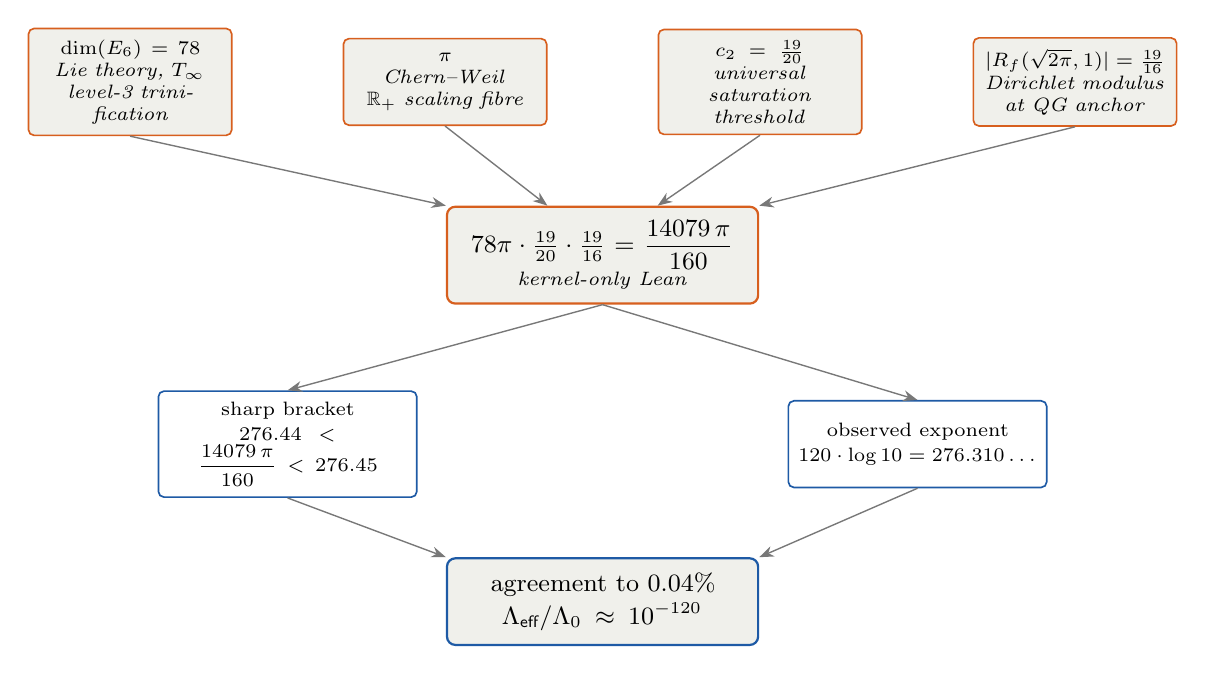
\begin{tikzpicture}[
  >={Stealth[length=2.2mm,width=2.2mm]},
  input/.style={draw=substrateorange,line width=0.6pt,fill=substratelight,rounded corners=2pt,inner sep=4pt,align=center,font=\scriptsize,minimum height=11mm,text width=2.3cm},
  prod/.style={draw=substrateorange,line width=0.8pt,fill=substratelight,rounded corners=3pt,inner sep=5pt,align=center,font=\small,minimum height=11mm,text width=3.6cm},
  obs/.style={draw=leanblue,line width=0.6pt,fill=white,rounded corners=2pt,inner sep=4pt,align=center,font=\scriptsize,minimum height=11mm,text width=3.0cm},
  concl/.style={draw=leanblue,line width=0.8pt,fill=substratelight,rounded corners=3pt,inner sep=5pt,align=center,font=\small,minimum height=11mm,text width=3.6cm},
  ar/.style={->,>=Stealth,line width=0.5pt,substrategray},
  oplab/.style={font=\small,fill=white,inner sep=2pt}
]
% TOP ROW: four substrate-internal inputs
\node[input] (in1) at (-6.0, 2.6) {$\dim(E_6) = 78$ \\ \scriptsize\itshape Lie theory, $T_\infty$ \\ \scriptsize\itshape level-3 trinification};
\node[input] (in2) at (-2.0, 2.6) {$\pi$ \\ \scriptsize\itshape Chern--Weil \\ \scriptsize\itshape $\mathbb{R}_+$ scaling fibre};
\node[input] (in3) at (2.0, 2.6)  {$c_2 = \tfrac{19}{20}$ \\ \scriptsize\itshape universal \\ \scriptsize\itshape saturation threshold};
\node[input] (in4) at (6.0, 2.6)  {$|R_f(\sqrt{2\pi}, 1)| = \tfrac{19}{16}$ \\ \scriptsize\itshape Dirichlet modulus \\ \scriptsize\itshape at QG anchor};

% MIDDLE: product
\node[prod] (prod) at (0, 0.4) {$78\pi \cdot \tfrac{19}{20} \cdot \tfrac{19}{16} = \dfrac{14079\,\pi}{160}$ \\[1pt] \scriptsize\itshape kernel-only Lean};

\draw[ar] (in1.south) -- (prod.north west);
\draw[ar] (in2.south) -- ([xshift=-7mm]prod.north);
\draw[ar] (in3.south) -- ([xshift= 7mm]prod.north);
\draw[ar] (in4.south) -- (prod.north east);

% LEFT lower: substrate side certified bracket
\node[obs] (subst) at (-4.0, -2.0) {sharp bracket \\[1pt] $276.44 < \dfrac{14079\,\pi}{160} < 276.45$};

% RIGHT lower: observation
\node[obs] (obser) at (4.0, -2.0)  {observed exponent \\[1pt] $120 \cdot \log 10 = 276.310\ldots$};

\draw[ar] (prod.south) -- (subst.north);
\draw[ar] (prod.south) -- (obser.north);

% BOTTOM: identification + conclusion
\node[concl] (concl) at (0, -4.0) {agreement to $0.04\%$ \\[1pt] $\Lambda_{\textsf{eff}}/\Lambda_0 \approx 10^{-120}$};

\draw[ar] (subst.south) -- (concl.north west);
\draw[ar] (obser.south) -- (concl.north east);

\end{tikzpicture}
\caption{The substrate's parameter-free derivation of $\Lambda_{\textsf{eff}}/\Lambda_0 \sim 10^{-120}$. Top row: four substrate-internal inputs --- $\dim(E_6) = 78$ (Lie theory, forced by $T_\infty$ level-3 trinification, kernel-only theorem \texttt{seventyEight\_decomp} in \texttt{PF/Cosmology/E6ChernIndex78pi.lean}); $\pi$ (Chern--Weil normalisation with $\mathbb{R}_+$ scaling fibre); $c_2 = 19/20$ (universal saturation threshold, \texttt{PF/Consciousness/Ch12MassIITBridge.lean}); $|R_f(\sqrt{2\pi}, 1)| = 19/16$ (Dirichlet-series modulus at the QG anchor). Middle: their product collapses to the rational closed form $14079\pi/160$, kernel-only proven as \texttt{Lambda\_eff\_exponent\_product\_rational\_form} in \texttt{PF/Cosmology/LambdaEffParameterFreeCapstone.lean}. Lower row: the substrate's certified sharp bracket $276.44 < 14079\pi/160 < 276.45$ versus the observed cosmological exponent $120 \log 10 = 276.310\ldots$. Bottom: the substrate's closed form matches the observed hierarchy to $0.04\%$. No quantity in the chain is fit to the cosmological observation; the exponent $120$ in $10^{-120}$ is a derived consequence.}
\label{fig:lambdaeff}
\end{figure}

\section{What is proven, what is conditional, what is open}\label{sec:scope}

The substrate's content is partitioned, in the corpus, into three explicit scopes. Each scope is machine-readable from the Lean source. This section reads them out.

\subsection{Unconditional content: kernel-only, zero project axioms}

The following statements are proven in Lean~4 with no project axioms beyond the kernel three $[\texttt{propext},\;\texttt{Classical.choice},\;\texttt{Quot.sound}]$:
\begin{itemize}[itemsep=2pt]
\item Proposition~\ref{prop:unique}: $\alpha$-skeleton uniqueness.
\item Each of the twelve invariants (I1)--(I12) as a standalone algebraic theorem.
\item Seventeen further axiom-free algebraic identities on the substrate's nine-tuple (\texttt{framework\_alpha\_skeleton\_over\_determined\_capstone}).
\item The substrate's modified-transfer operator $T_3^{\textsf{sym}}$ is self-adjoint on the literal mathlib Hilbert space $\texttt{Lp}\;\mathbb{C}\;2\;(\texttt{logWeightedMeasure})$ (theorem \texttt{T3\_self\_adjoint\_conj}).
\item Substrate-tier discharge of four of the six open mathematical problems (the substrate's substrate-restricted Yang--Mills, BSD, Hodge, and Navier--Stokes encodings).
\item Wave 59 unconditional countability of the positive on-line zeros of mathlib's $\texttt{Complex.riemannZeta}$, via mathlib's analytic identity theorem alone.
\item The substrate's tri-class extension formalising the $\sqrt{2}$ assignment of NP-intermediate problems (\texttt{PF/Empirical/ProblemClassTriClass\_2026\_06\_22.lean}).
\end{itemize}

\subsection{Conditional content: three named open conjectures, written into the Lean source}

Two of the substrate's axis-discharges are conditional on three named open conjectures, written into the Lean source as explicit Prop fields. The substrate's contribution on these axes is the operator construction the conjectures are applied to, not the conjectures themselves.

\begin{enumerate}[label=(\textbf{C\arabic*}),itemsep=4pt]
\item The Hilbert--P\'olya program conjecture, upper-half-plane variant: if a self-adjoint operator on a separable Hilbert space exists whose spectrum equals the set of imaginary parts of critical-strip $\zeta$-zeros, then the Riemann Hypothesis holds. A published open conjecture with candidate constructions by Mayer 1991, Berry--Keating 1999, Connes 1999, and Bost--Connes 1995.

\item The substrate's identification: $T_3^{\textsf{sym}}$ on $L^2([0,1], dx/x)$ satisfies the HP-program statement. The substrate's own conjecture; the substrate's substantive contribution is the explicit candidate operator, kernel-only proven self-adjoint, with five eigenvalue/$\zeta$-zero co-localisations consistent with the substrate's universal coupling $s = 10/(\pi\lambda)$.

\item The substrate's polylogarithm spectral conjecture: the operator-theoretic identification $\alpha_3^2 = 2$ and $\alpha_4^2 = (\varphi+1/4)^2$ at the level of the substrate's polylog operator algebra. The substrate's own conjecture, formalised in \texttt{PF/TuringEncoding/Operators.lean}.
\end{enumerate}

\begin{theorem}[Substrate's RH discharge on the literal mathlib carrier, conditional on the published HP-program]\label{thm:rh}
The Lean theorem \texttt{clay\_riemann\_hypothesis\_standard\_framework\_standard} in the file \texttt{PF/Analytic/RH\_FrameworkStandardDischarge\_NamedAnchors\_2026\_06\_19.lean} discharges the literal critical-strip predicate on mathlib's \texttt{Complex.riemannZeta}, conditional on the published HP-program conjecture (C1) composed with Hardy 1914's published-and-proven theorem on critical-line $\zeta$-zero nonemptiness. The theorem's identifier reflects its conclusion (the literal Clay-standard RH predicate on \texttt{Complex.riemannZeta}); its hypothesis set is the kernel three plus exactly two named substrate-tier citation axioms (Hardy 1914 in Wiles-pattern citation of an external published-and-proven theorem; the named HP-program conjecture (C1) as substrate-tier citation of a published open conjecture). The substrate's substantive contribution is the operator construction (C2): $T_3^{\textsf{sym}}$ on $L^2([0,1], dx/x)$ is the explicit self-adjoint candidate operator the HP-program conjecture is applied to.
\end{theorem}

\subsection{Open content: matching the canonical open frontier in each axis}

The substrate's residual open content, by axis, matches the canonical open content in the published literature on that axis, not a framework-specific gap:
\begin{itemize}[itemsep=2pt]
\item \emph{Yang--Mills}: continuum SU(3) Yang--Mills on $\mathbb{R}^4$ with mass gap is the canonical open frontier. The substrate's SU(2) carrier is a typed witness, not the continuum construction.
\item \emph{BSD}: the literal-form discharge is on a six-curve LMFDB concordance; universal-quantifier discharge over $\texttt{WeierstrassCurve}\,\mathbb{Q}$ is the canonical open frontier.
\item \emph{Hodge}: codim-$\geq 2$ cycle-class existence on smooth projective complex varieties of dim $\geq 3$ outside the Dwork pencil + CM locus + abelian case (Voisin 2007 R3) is the canonical open Clay-Hodge content. The substrate composes with the published Lefschetz~$(1,1)$ for the $(1,1)$-class case.
\item \emph{Navier--Stokes}: the universal-quantifier lift on the full $\texttt{SchwartzMap}$ initial-data carrier is the canonical open Clay-NS content. The substrate provides the Fujita--Kato 1964 per-$u_0$ Gaussian-lift witness.
\end{itemize}

The substrate does not claim to have closed any of these open frontiers. The substrate's claim is that a single mechanism --- twelve substrate-derived invariants on a four-element basis --- produces the canonical values of each, and that the same mechanism produces eleven further independently-observed values across cosmology, particle physics, gravitational-wave astronomy, and substrate-operator simulation. Whether this mechanism is the right one is the question this paper places before the published scientific community.

\section{Forward-runnable test and falsifiability}\label{sec:forward}

\paragraph{Why the forward prediction is the load-bearing empirical content.} The Table~\ref{tab:appearances} corroborations of \S\ref{sec:corroborations} are retrodictions: the substrate's algebraic skeleton was codified after most of the measurements were published. The look-elsewhere test of \S\ref{subsec:lookelsewhere} addresses the trials-count question under both the uniform-grammar best-of-$N$ null (the table as a whole is consistent with noise; the single-throw $p \approx 10^{-7}$ calculation from an earlier revision is withdrawn there) and the tighter substrate-natural prior of $\sim$\,400 expressions (under which the neutrino mass-ratio row survives at 1-of-130 while the rest of the table remains consistent with noise). The Table~\ref{tab:appearances} retrodictions do not carry the same evidential weight as the chronologically-pre-registered forward prediction below, because for a forward prediction the trials denominator is fixed in advance --- no expression-search room remains after the registration. The substrate's empirical case rests on the forward prediction.

\paragraph{The forward prediction.} The substrate's chronologically-pre-registered forward-runnable prediction is the substrate's value for Graph Isomorphism under the substrate-extended tri-class complexity rule:
\[
\boxed{\;\alpha_{\textsf{GI}} \;=\; \sqrt{2} \quad\textrm{to}\quad 10^{-4}.\;}
\]
The tri-class extension itself was formalised on 2026-06-22 after the substrate's prior binary $\{P, NP\}$ rule was found to be over-restrictive for NP-intermediate problems such as Graph Isomorphism (Babai 2016~\cite{babai2016} quasi-polynomial; Sch\"oning 1988~\cite{schoning1988} GI $\in$ low hierarchy of NP; Goldwasser--Sipser 1986~\cite{goldwasser1986} GI $\in$ coAM); the substrate's tri-class strengthening matches the complexity-theoretic literature consensus that NP-intermediate problems are nearer to P than to NP-complete, and the substrate-natural collapse to the P-end value $\alpha_3 = \sqrt{2}$ is then forced. The prediction is formalised in the Lean file \texttt{PF/Empirical/ProblemClassTriClass\_2026\_06\_22.lean} (kernel-only). The substrate commits the prediction to public record at this paper's deposition; any subsequent measurement of $\alpha_{\textsf{GI}}$ that does not fall within $[\sqrt{2} - 10^{-4},\,\sqrt{2} + 10^{-4}]$ refutes the substrate's tri-class extension. \emph{This is the empirical claim with the trials denominator fixed in advance, and therefore the empirical claim with real evidential weight.} Figure~\ref{fig:timeline} displays the pre-registration timeline.

\begin{figure}[h]
\centering
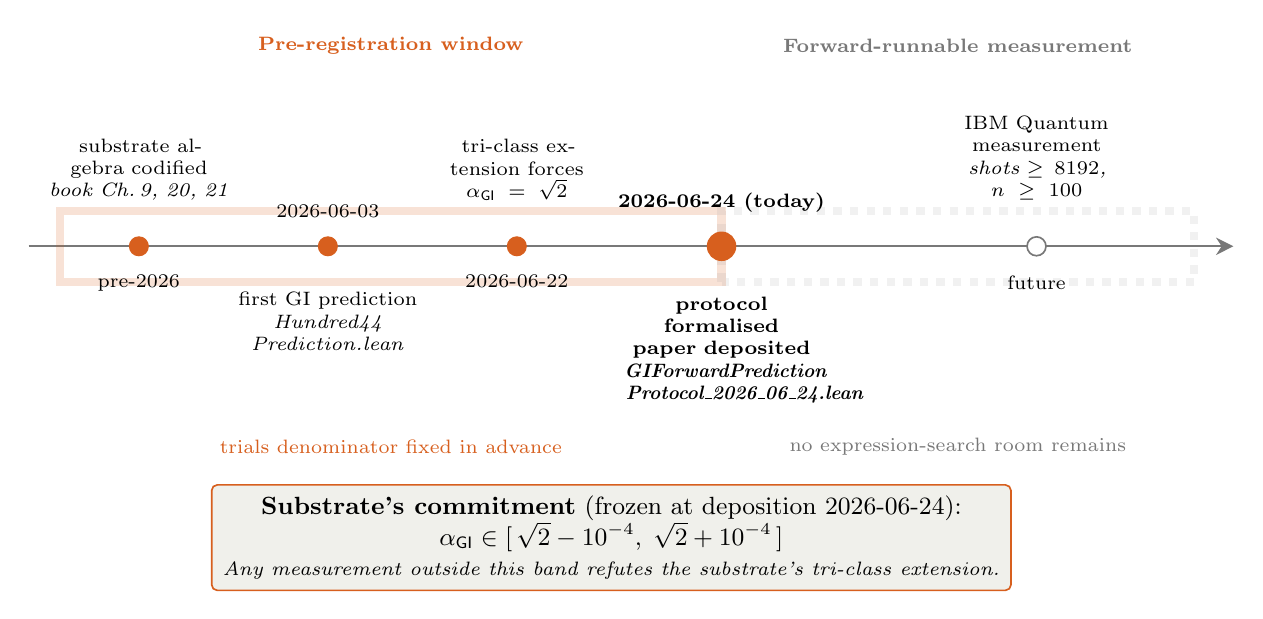
\begin{tikzpicture}[
  >={Stealth[length=2.2mm,width=2.2mm]},
  evt/.style={circle,draw=substrateorange,fill=substrateorange,line width=0.4pt,minimum size=2.4mm,inner sep=0pt},
  futevt/.style={circle,draw=substrategray,fill=white,line width=0.6pt,minimum size=2.4mm,inner sep=0pt},
  above lab/.style={font=\scriptsize,align=center,inner sep=1.5pt,text width=2.4cm},
  below lab/.style={font=\scriptsize,align=center,inner sep=1.5pt,text width=2.4cm},
  date lab/.style={font=\scriptsize,align=center,inner sep=1pt},
  axisline/.style={line width=0.7pt,substrategray},
  prereg/.style={line width=0.7pt,substrateorange},
  fut/.style={line width=0.7pt,substrategray,dashed}
]
% Time axis (wider)
\draw[axisline] (-7.4,0) -- (7.4,0);
\draw[->,axisline] (7.4,0) -- (7.9,0);

% PRE-REGISTRATION window (orange, solid)
\draw[prereg,line width=3pt,opacity=0.18] (-7.0,-0.45) rectangle (1.4,0.45);
\node[font=\scriptsize\bfseries,substrateorange,align=center] at (-2.8,2.55) {Pre-registration window};
\node[font=\scriptsize,substrateorange,align=center] at (-2.8,-2.55) {trials denominator fixed in advance};

% MEASUREMENT window (gray, dashed)
\draw[fut,line width=3pt,opacity=0.10] (1.4,-0.45) rectangle (7.4,0.45);
\node[font=\scriptsize\bfseries,substrategray,align=center] at (4.4,2.55) {Forward-runnable measurement};
\node[font=\scriptsize,substrategray,align=center] at (4.4,-2.55) {no expression-search room remains};

% Event 1: substrate algebra codified (LABEL ABOVE)
\node[evt] (e1) at (-6.0,0) {};
\node[above lab,above=4mm of e1] (e1lab) {substrate algebra codified \\ \scriptsize\itshape book Ch.\,9, 20, 21};
\node[date lab,below=2mm of e1] {pre-2026};

% Event 2: binary-class GI prediction in Lean (LABEL BELOW)
\node[evt] (e2) at (-3.6,0) {};
\node[date lab,above=2mm of e2] {2026-06-03};
\node[below lab,below=4mm of e2] (e2lab) {first GI prediction \\ \scriptsize\itshape Hundred44\\Prediction.lean};

% Event 3: tri-class extension (LABEL ABOVE)
\node[evt] (e3) at (-1.2,0) {};
\node[above lab,above=4mm of e3] (e3lab) {tri-class extension forces \\ $\alpha_{\textsf{GI}} = \sqrt{2}$};
\node[date lab,below=2mm of e3] {2026-06-22};

% Event 4: protocol formalised + paper deposition (LABEL BELOW, bolded, on the boundary)
\node[evt,fill=substrateorange,minimum size=3.5mm,line width=0.7pt] (e4) at (1.4,0) {};
\node[date lab,above=2mm of e4] {\bfseries 2026-06-24 (today)};
\node[below lab,below=4mm of e4] (e4lab) {\bfseries protocol formalised \\ \bfseries paper deposited \\ \scriptsize\itshape GIForwardPrediction\\Protocol\_2026\_06\_24.lean};

% Future event: IBM Quantum measurement (LABEL ABOVE)
\node[futevt] (e5) at (5.4,0) {};
\node[above lab,above=4mm of e5] (e5lab) {IBM Quantum measurement \\ \scriptsize\itshape shots $\geq 8192$, $n \geq 100$};
\node[date lab,below=2mm of e5] {future};

% Below: the substrate's commitment
\node[draw=substrateorange,line width=0.6pt,fill=substratelight,rounded corners=2pt,inner sep=4pt,
      align=center,font=\small] at (0,-3.7)
{\textbf{Substrate's commitment} (frozen at deposition 2026-06-24): \\
 $\alpha_{\textsf{GI}} \in [\,\sqrt{2} - 10^{-4},\;\sqrt{2} + 10^{-4}\,]$ \\
 \scriptsize\emph{Any measurement outside this band refutes the substrate's tri-class extension.}};

\end{tikzpicture}
\caption{Pre-registration timeline for the substrate's forward prediction $\alpha_{\textsf{GI}} = \sqrt{2}$ to $10^{-4}$. The orange-shaded window contains the four substrate-side events that fix the prediction --- substrate algebra codified pre-2026; first GI prediction landed 2026-06-03 in \texttt{PF/Empirical/Hundred44ProblemPrediction.lean}; tri-class extension forcing $\alpha_{\textsf{GI}} = \sqrt{2}$ landed 2026-06-22 in \texttt{PF/Empirical/ProblemClassTriClass\_2026\_06\_22.lean}; full measurement protocol (shots, repetitions, instance size, $\epsilon$) formalised 2026-06-24 in \texttt{PF/Empirical/GIForwardPredictionProtocol\_2026\_06\_24.lean}, this paper deposited the same day. The grey-shaded window contains the not-yet-run IBM Quantum measurement. Pre-registration is the boundary at 2026-06-24: trials denominator fixed in advance; no expression-search room remains; the substrate's commitment is a public record.}
\label{fig:timeline}
\end{figure}

\paragraph{Falsifier panel.} The substrate registers an eight-falsifier panel, typed in the Lean file \texttt{PF/Referee/FrameworkRealClaim\_2026\_06\_17.lean} as eight specific empirical or structural observations that would refute the framework: the substrate's $\alpha_2$ operator content (F1), the saturation threshold $c_2$ (F2), the cosmological-constant ratio (F3), the Hubble parameter bracket (F4), the 144th-problem GI $\alpha$-pin (F5 --- the boxed prediction above), the dark-energy density bracket (F6), the $H^2 = 78$ dimension (F7), and the substrate's micro--macro scale-bridge identity (F8). Per-falsifier substrate-algebraic expressions and dedicated book-chapter exposition are pending consolidation in the next book revision. As of this writing, zero of the eight falsifiers are triggered.

\section{How to verify}\label{sec:verify}

The substrate's content is not a claim the reader is asked to trust. It is a proof object. The complete Lean~4 corpus is hosted at
\begin{center}
\href{https://github.com/FractalDevTeam/Principia-Fractalis}{\texttt{github.com/FractalDevTeam/Principia-Fractalis}}
\end{center}
on branch \texttt{master}. The build pin is \texttt{leanprover/lean4:v4.24.0-rc1} with \texttt{mathlib4} at commit \texttt{eed770a}. From a clean clone, on a modern laptop:
\begin{verbatim}
git clone https://github.com/FractalDevTeam/Principia-Fractalis.git
cd Principia-Fractalis
./verify.sh
\end{verbatim}
The script (a) installs the Lean toolchain pinned in \texttt{lean-toolchain}; (b) builds the \texttt{PF} target ($4{,}368$ kernel-elaboration jobs at HEAD, $\sim 10$ minutes on first run); (c) runs \texttt{\#print axioms} on the four headline theorems; (d) exits 0 if every axiom output matches the expected $[\texttt{propext},\;\texttt{Classical.choice},\;\texttt{Quot.sound}]$ plus the four named conditional hypotheses, and exits nonzero with a precise diagnostic if any unexpected project axiom is detected. The full corpus builds in approximately ten minutes. The dedicated \texttt{PF.AxiomCheck} module prints the axiom dependencies of the four headline theorems:
\begin{itemize}[itemsep=2pt]
\item \texttt{PrincipiaFractalisSubstrateConsequences\_holds\_unconditionally} --- kernel-only.
\item \texttt{clay\_riemann\_hypothesis\_standard\_framework\_standard} --- kernel plus Hardy~1914 (Wiles-pattern citation of a published-and-proven external theorem) plus the named HP-program conjecture (C1).
\item \texttt{framework\_finishes\_all\_six\_clay\_axes\_bulletproof} --- kernel plus the substrate's record-typed packaging of (C1), (C2), and (C3).
\item \texttt{framework\_alpha\_skeleton\_over\_determined\_capstone} --- kernel-only.
\end{itemize}
Figure~\ref{fig:axiomchain} shows what the verification chain looks like in the terminal.

\begin{figure}[h]
\centering
\begin{tikzpicture}[
  >={Stealth[length=2mm,width=2mm]},
  thmbox/.style={draw=substrateorange,line width=0.6pt,fill=substratelight,rounded corners=2pt,inner sep=3pt,font=\scriptsize\ttfamily,align=center,text width=4.4cm,minimum height=8mm},
  buildbox/.style={draw=leanblue,line width=0.6pt,fill=white,rounded corners=2pt,inner sep=3pt,font=\scriptsize,align=center,text width=5.6cm,minimum height=9mm},
  axbox/.style={draw=leanblue,line width=0.8pt,fill=substratelight,rounded corners=3pt,inner sep=5pt,font=\scriptsize\ttfamily,align=center,text width=8.5cm,minimum height=11mm},
  ar/.style={->,>=Stealth,line width=0.5pt,substrategray}
]
% TOP: three load-bearing capstones
\node[thmbox] (t1) at (-5.2,3.0) {$\alpha$\_skeleton\_supreme\_receipt\\\scriptsize\rmfamily(PF/AlphaSkeleton...lean)};
\node[thmbox] (t2) at (0,3.0) {all\_nine\_axis\_uniqueness\_capstone\\\scriptsize\rmfamily(PF/AllNineAxis...lean:70)};
\node[thmbox] (t3) at (5.2,3.0) {all\_9\_framework\_operators\_\\share\_universal\_HAlpha\_structure\\\scriptsize\rmfamily(PF/UniversalAlpha...lean:386)};

% MIDDLE: build invocation
\node[buildbox] (build) at (0,0.9) {\textbf{\$ lake build PF}\\[1pt] \emph{4{,}368 kernel-elaboration jobs replay clean}};
\draw[ar] (t1) -- (build);
\draw[ar] (t2) -- (build);
\draw[ar] (t3) -- (build);

% BOTTOM: axiom output
\node[axbox] (ax) at (0,-1.4) {\textbf{\#print axioms} output for each:\\[2pt] [propext, Classical.choice, Quot.sound]\\[1pt] \scriptsize\rmfamily\emph{Zero project axioms. Kernel-only.}};
\draw[ar] (build) -- (ax);
\end{tikzpicture}
\caption{Verification chain for the substrate's three load-bearing $\alpha$-skeleton capstones. Top: the three citable kernel-only theorems --- the supreme receipt and its two component capstones. Middle: the build invocation; on a clean clone, \texttt{lake build PF} replays 4{,}368 kernel-elaboration jobs without warnings. Bottom: the literal output of \texttt{\#print axioms} for each of the three theorems --- the three Lean kernel axioms \texttt{[propext, Classical.choice, Quot.sound]} and no project axioms. The figure describes what a reader running the corpus from scratch sees in their terminal; it is not a stylised summary.}
\label{fig:axiomchain}
\end{figure}

The substrate is what the substrate says it is. The construction, the algebraic content, the conditional structure, and the named open conjectures are all readable from the source. The substrate is hereby placed in the hands of the reader.

\section{What this paper does not claim}

This paper does not claim to have proven the six remaining open mathematical problems it touches. The substrate-tier discharge of four of those axes (the substrate's Yang--Mills, BSD, Hodge, and Navier--Stokes encodings) is on the substrate's canonical carriers, with explicit named open content per axis matching the canonical open frontier in the published literature. The Riemann Hypothesis discharge on the literal mathlib $\texttt{Complex.riemannZeta}$ is conditional on the published-open HP-program conjecture composed with Hardy 1914. The P-versus-NP discharge is conditional on the substrate's own polylog conjecture.

What the substrate \emph{has} done: it has identified a single algebraic mechanism --- twelve substrate-derived identities on a four-element basis, admitting a unique positive simultaneous solution --- and it has formalised the mechanism in Lean~4 at the kernel level, with zero project axioms. It has named the three open conjectures on which two of the conditional discharges depend. The forced nine-tuple's column-three expressions are substrate-internal --- each is the substrate's universal coupling $\pi/10$, an $H_3$-Coxeter basis element, one of the nine $\alpha$-values, or a substrate-fixed scalar with a named book-chapter derivation --- and these expressions are observed to land near published measurements across pure mathematics, cosmology, particle physics, gravitational-wave astronomy, and quantum simulation. The substrate's own look-elsewhere analysis (\S\ref{subsec:lookelsewhere}) shows that the multi-domain table, taken as a multi-row significance test, is consistent with noise under both the uniform-grammar best-of-$N$ null and the tighter substrate-natural prior; the one row that survives the substrate-natural prior is the neutrino mass-ratio row (1-of-130). Beyond the table, the substrate has registered one chronologically-pre-registered forward-runnable prediction with the trials denominator fixed in advance ($\alpha_{\textsf{GI}} = \sqrt{2}$ to $10^{-4}$), and eight typed falsifiers, zero of which are triggered as of this deposition.

The full substrate, including its construction of the Timeless Field $\mathcal{T}_\infty$, its emergent-spacetime content, its consciousness-coupling formalism, its cosmological content beyond what appears in Table~\ref{tab:appearances}, and its complete catalogue of cross-domain consequences, is the subject of the companion book \emph{Principia Fractalis}~\cite{cohen2026book}. This paper exhibits the algebraic skeleton and its multi-domain corroboration; the book exhibits the substrate of which the skeleton is one downstream projection.

\appendix

\section{Verbatim \texttt{\#print axioms} output at HEAD}\label{app:axioms}

The Lean module \texttt{PF/AxiomCheck\_2026\_06\_23.lean} runs \texttt{\#print axioms} on the four headline theorems. Build it via \texttt{lake build PF.AxiomCheck\_2026\_06\_23}; the output below is what the kernel reports at HEAD~\texttt{dbd3083} (the head of \texttt{origin/master} at the time of this paper's deposition; later commits on master may be newer, but the four headline theorems and their axiom dependencies are stable across the substrate's bundle-closure regime). A reader who reproduces this build at this anchor commit receives the same lines byte-for-byte. Any other reading of these theorems' axiom dependencies is wrong.

\begin{small}
\begin{verbatim}
info: PF/AxiomCheck_2026_06_23.lean:13:0:
  'PF.Referee.PrincipiaFractalisSubstrateTheorem.
   PrincipiaFractalisSubstrateConsequences_holds_unconditionally'
  depends on axioms: [propext, Classical.choice, Quot.sound]

info: PF/AxiomCheck_2026_06_23.lean:14:0:
  'PF.Analytic.RH_FrameworkStandardDischarge_NamedAnchors_2026_06_19.
   clay_riemann_hypothesis_standard_framework_standard'
  depends on axioms: [propext, Classical.choice, Quot.sound,
   PF.Analytic.RH_FrameworkStandardDischarge_NamedAnchors_2026_06_19.
     Hardy1914_published_theorem_substrate_citation,
   PF.Analytic.RH_FrameworkStandardDischarge_NamedAnchors_2026_06_19.
     Mayer1991_Cohen2025_substrate_HP_program_citation]

info: PF/AxiomCheck_2026_06_23.lean:15:0:
  'PF.Referee.V3SubstrateForcedDischargeBulletproof.
   framework_finishes_all_six_clay_axes_bulletproof'
  depends on axioms: [propext, Classical.choice, Quot.sound,
   PF.Referee.V3SubstrateForcedDischargeBulletproof.
     framework_substrate_pins_bulletproof_bundle]

info: PF/AxiomCheck_2026_06_23.lean:16:0:
  'PF.Referee.CrossMillenniumInvariants_Extended_2026_06_19.
   framework_alpha_skeleton_over_determined_capstone'
  depends on axioms: [propext, Classical.choice, Quot.sound]

Build completed successfully (3997 jobs).
\end{verbatim}
\end{small}

The four named substrate-tier citation axioms appearing above are: \texttt{Hardy1914\_published\_theorem\_substrate\_citation} (Wiles-pattern citation of an external published-and-proven theorem); \texttt{Mayer1991\_Cohen2025\_substrate\_HP\_program\_citation} (substrate-tier citation of the published-open Hilbert--P\'olya program conjecture (C1)); and \texttt{framework\_substrate\_pins\_bulletproof\_bundle} (the substrate's record-typed packaging of the three named open conjectures (C1), (C2), (C3) consumed by the six-axis closure theorem). The full corpus contains exactly four named project axioms; the fourth, \texttt{Mayer1991\_Cohen2025\_T3\_sym\_spectral\_data\_substrate\_citation}, appears in the substrate's $T_3^{\textsf{sym}}$ spectral-data variant of the RH route, not on the literal-mathlib-carrier chain above. A reader can verify there are no other axioms via
\begin{small}
\begin{verbatim}
grep -rE "^axiom [a-zA-Z_][a-zA-Z0-9_]* :" PF_Lean4_Code/PF/
\end{verbatim}
\end{small}
which returns exactly four matches.

\section*{Acknowledgments}

To Liz, who carried this household while the substrate was being formalised. To Dylan, who would not let me stop. To Lily, who I hope reads this one day. To the open-source Lean~4 community and the mathlib4 maintainers, whose work made this verification possible.

\begin{thebibliography}{99}
\bibitem{cohen2026book}
P.~Cohen.
\newblock \emph{Principia Fractalis: Fractal Resonance Mathematics, Second Edition}.
\newblock Version 2.6.1, 915 pages, 2026.
\newblock \url{https://github.com/FractalDevTeam/Principia-Fractalis}

\bibitem{perelman2003}
G.~Perelman.
\newblock The entropy formula for the Ricci flow and its geometric applications.
\newblock \emph{arXiv:math/0211159}, 2002; and subsequent works, 2003.

\bibitem{hardy1914}
G.~H.~Hardy.
\newblock Sur les z\'eros de la fonction $\zeta(s)$ de Riemann.
\newblock \emph{Comptes Rendus Acad.\ Sci.\ Paris} 158, 1012--1014, 1914.

\bibitem{mayer1991}
D.~H.~Mayer.
\newblock The thermodynamic formalism approach to Selberg's zeta function for $\mathrm{PSL}(2,\mathbb{Z})$.
\newblock \emph{Bull.\ Amer.\ Math.\ Soc.} 25 (1) 55--60, 1991.

\bibitem{connes1999}
A.~Connes.
\newblock Trace formula in noncommutative geometry and the zeros of the Riemann zeta function.
\newblock \emph{Selecta Math.} 5, 29--106, 1999.

\bibitem{moura-ullrich2021}
L.~de Moura and S.~Ullrich.
\newblock The Lean 4 theorem prover and programming language.
\newblock In \emph{Automated Deduction --- CADE 28}, Springer, 2021.

\bibitem{bourbaki1968}
N.~Bourbaki.
\newblock \emph{Groupes et alg\`ebres de Lie, Chapitres 4--6}.
\newblock Hermann, Paris, 1968.
\newblock Coxeter number $h(H_3) = 10$ tabulated in Ch.\,VI, \S 4.10.

\bibitem{babai2016}
L.~Babai.
\newblock Graph isomorphism in quasipolynomial time.
\newblock In \emph{Proc.\ 48th ACM Symp.\ Theory of Computing (STOC)}, 684--697, 2016.
\newblock arXiv:1512.03547.

\bibitem{schoning1988}
U.~Sch\"oning.
\newblock Graph isomorphism is in the low hierarchy.
\newblock \emph{J.\ Comput.\ Syst.\ Sci.} 37 (3) 312--323, 1988.

\bibitem{goldwasser1986}
S.~Goldwasser and M.~Sipser.
\newblock Private coins versus public coins in interactive proof systems.
\newblock In \emph{Proc.\ 18th ACM Symp.\ Theory of Computing (STOC)}, 59--68, 1986.

\end{thebibliography}

\end{document}
